\chapter{Evaluation}
\label{cha:evaluation}
This last chapter presents how the prototype have been evaluated to observe if and how it meets the initial research question.
Performance evaluation for the classifiers is presented. Finally, the Section~\ref{sec:InsAct} explains how the extracted insights can impact a business and help it in the interaction with its customers.

On the one hand, classifiers for the four dimensions of the MBTI personality model were evaluated using confusion matrices.
A confusion matrix is a $2x2$ table used to observe the results of a binary classification algorithm.
In general, along its columns it contains the values predicted by the machine learning algorithm. The rows represent the actual class of the samples. Figure~\ref{fig:confMat} shows how the table is structured.
The output of a binary classification can be either 0, or \textit{negative} class, or 1 \textit{positive} class.
So, the 4 cells of the matrix assume these names: at top-left there is the \textit{true positives} (TP) counter, the top-right is the counter for the \textit{false negative} (FN), the bottom-left one for the \textit{false positives} (FP), and bottom-right for \textit{true negative} (TN).
Totally, their sum is equal to the number of samples classified.
From this table, 4 measures as usually extracted: 

\begin{equation*}
\begin{split}
\text{Accuracy} & = \frac{TP + TN}{TP + TN + FP + FN}\\
\text{Precision} & = \frac{TP}{TP + FP} \\ 
\text{Recall} & = \frac{TP}{TP + FN}\\
\text{F}_1\text{-Score} & = 2 * \frac{\text{Precision} * \text{Recall}}{\text{Precision} + \text{Recall}}
\end{split}
\end{equation*}

\begin{figure}
\centering
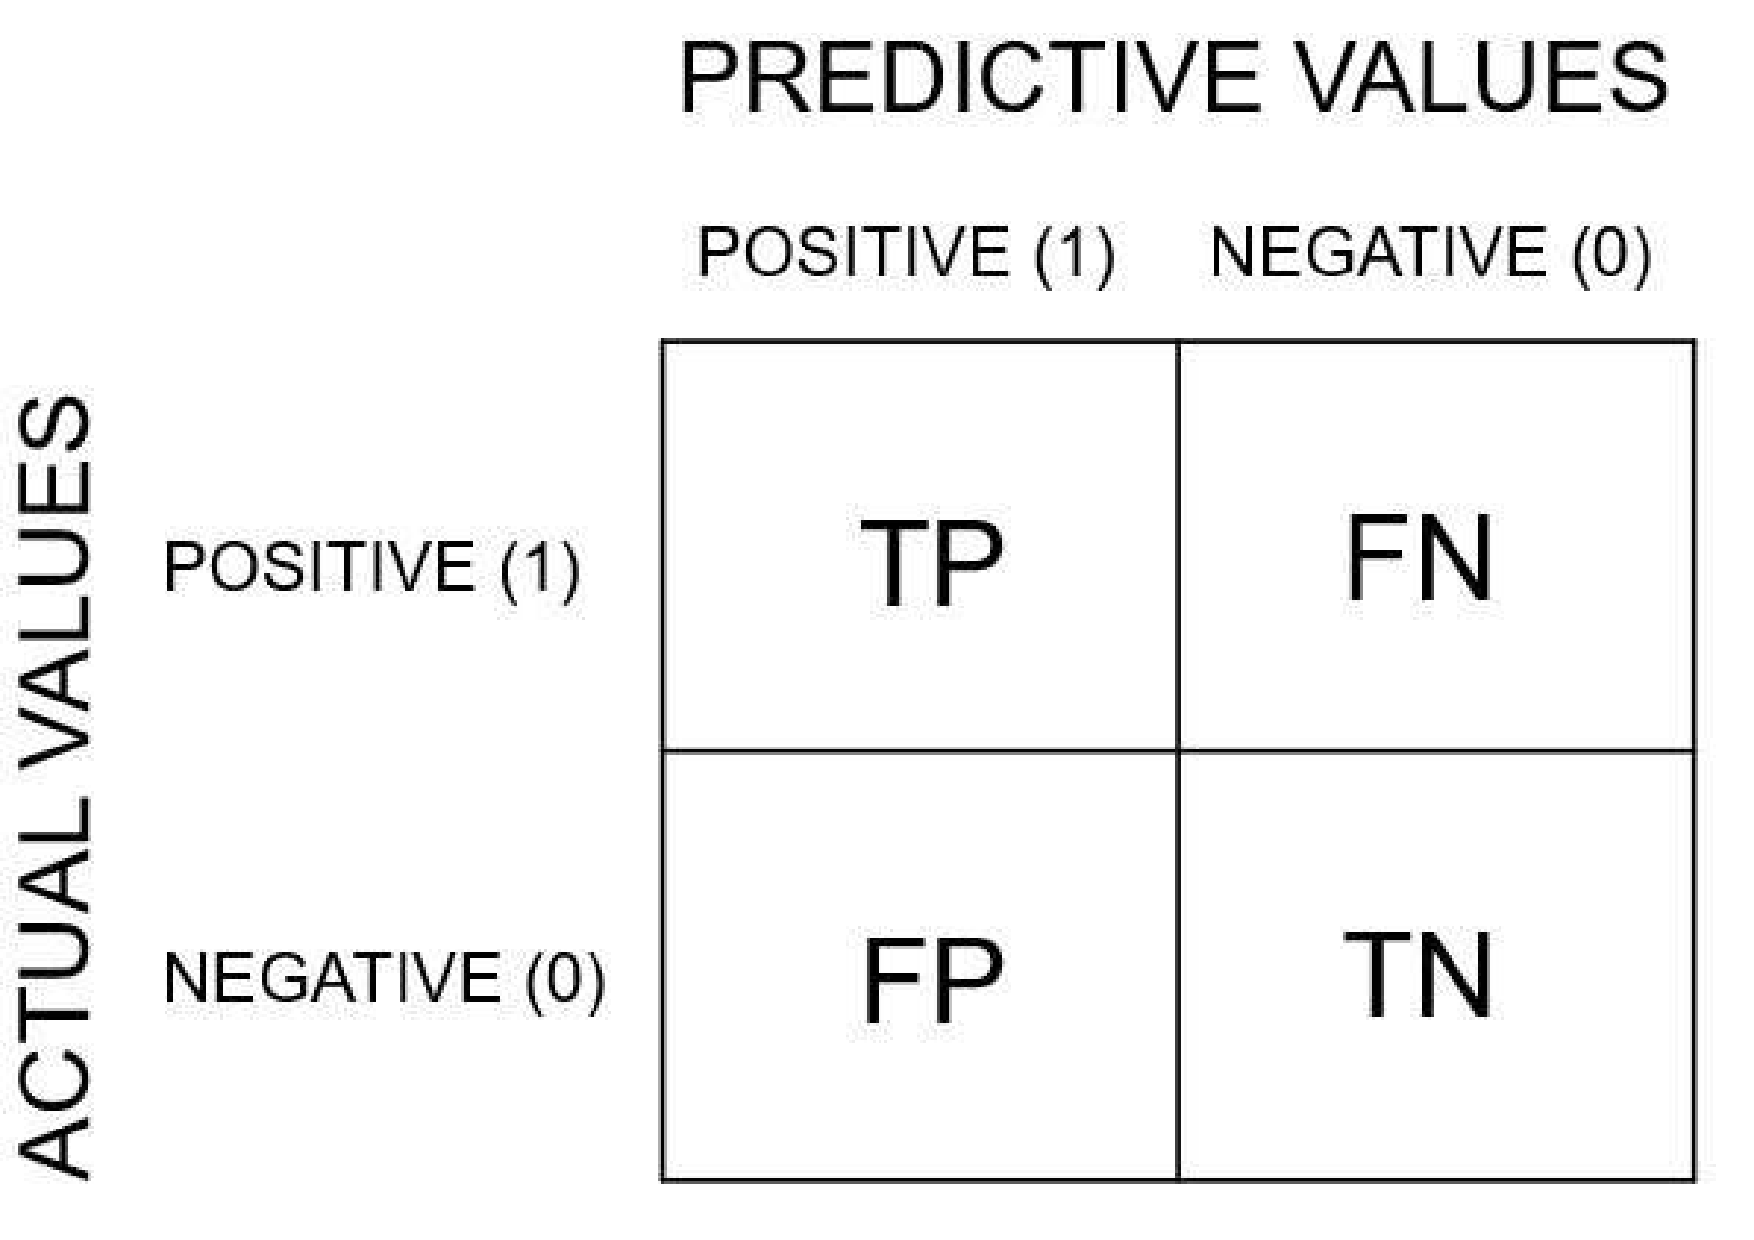
\includegraphics[width=%
0.7\textwidth,height=6.5cm,keepaspectratio]{img/confMatrix.pdf}
\caption{Generic schema of a confusion matrix}
\label{fig:confMat}
\end{figure}

\section{MBTI Classifiers evaluation}
Regarding these 4 classifiers, no particular setups have been applied.
Decision trees have been chosen as classifiers, according to the current stato of the art.
Naive bayes classifiers are also usually applied for such purposes but were discarded due to bad performance with the linguistic features.

The performance evaluations were performed on the same dataset used to train the four classifiers.
The dataset was split into a training set and a test one using the default values of the scikit-learn library. So, the training set contained $75\%$ of the samples and the test set the remaining $25\%$.
The used features include some information from the social profile, such as the number of followers and friends, the use of hashtags, mentions, and URLs, and other information describing the text component, such as the number of sentences and word and POS tags.
No particular configuration have been used for what regards \textit{bags of words} or \textit{n-grams}.

The measure observed to compare the performance with that of the current state of the art is the \textbf{accuracy}.
Accuracy is the ratio of correct prediction to total predictions made. It is presented as a percentage.
Accuracy is preferred since, for each of the four classifications, there is not discrimination between samples with a specific outcome from normal observation.
So, even though, taking as example the cognitive function \textit{Extroversion/Introversion}, extroversion is labelled as the negative class and introversion as the positive one, it is not the case where we want to reduce the number of false-positive rather than false-negative because both classes are treated the same way.
So, metrics such as precision or recall tend to be avoided and not considered in the state of the art.

Even though only standard methodologies have been applied, the classifiers had discrete results. 
Table~\ref{tab:results} compares the obtained results with that of the state of the art \cite{lima2019tecla}.
Compared to those obtained by Lima et al., the prototype's performances are slightly worse. 
It should be said that the study considered reached its best results using a particular set of psychological features extracted with services such as the \textit{Linguistic Inquire and Word Count} (LIWC).
But, as said in Section~\ref{sec:resObj}, this thesis focuses more on the actionability of the extracted insights rather than their accuracy and reliability.

\begin{table}[htbp]
    \centering
    \begin{tabular}{ccccc}
    \hline
    Classifiers & Extr/Intr & Sensation/Intuition & Think/Feel & Judging/Perceiving \\
    \hline
    \textbf{System accuracy} & $77.6\%$ & $81.8\%$ & $76.9\%$ & $74.3\%$ \\
    \textbf{SOA accuracy} & $82.0\%$ & $88.3\%$ & $80.57\%$ & $78.26\%$ \\
    \hline
    \end{tabular}
    \caption{Table.\label{tab:results}}
\end{table}

\section{Non-ML insights observation}
While for the four classifiers of the personality traits there is an availability of data for both the training and the evaluation of ML models, this is not possible for the other classifiers which are based on non-machine learning algorithms, described in Section~\ref{sec:Classifiers}.
To observe and evaluate their results, the user dashboard introduces in Section~\ref{sec:userDash} has been used.

To do it, nearly twenty twitter profiles were downloaded and classified for a total of more than forty thousand activities.
Their results have been displayed over time thanks to the batch-based architecture and then observed individually.

Some interesting observations can be done comparing the results for two, or more, different profiles.
For example, two of the downloaded profiles, which comes from a similar environment, are the one of the \textbf{University of Trento} (\url{https://twitter.com/UniTrento}) and that of the \textbf{Department of Information Engineering and Computer Science} (\url{https://twitter.com/UniTrento_DISI})

\section{Insights' actionability}
An important goal that this thesis aimed to meet was to extract actionable insights. Insights capable of helping a company during their interaction with its customers.
This short section gives some examples of how the implemented classifiers can actually help a business.

Starting with one of the four personality traits
\label{sec:InsAct}